\section{Conventions de code}
	Par soucis de réutilisabilité et de partage de notre projet, nous avons choisi d'utiliser l'anglais pour la documentation du code mais aussi pour le code en lui-même (nom de fonction, nom de variable, etc).


\section{Répartition du travail}
	La répartition du travail nous a été indirectement imposée par la structure du projet. 
	
	Tout d'abord la partie analyse du projet c'est fait par le groupe entier car
	l'analyse c'est la base d'un projet, donc nous avons choisi de la faire tous ensemble pour essayer d'avoir une analyse représentative du groupe et plus poussée. Comme le projet est divisé en deux parties, la partie développement \gls{android} et la partie \gls{ios}, de ce fait comme seulement Kilian Cousein et Benjamin Tardieu posséder un Macintosh, ces derniers ont développés la partie iOS et l'autre partie à été développée part Olivier Bonvila et Ludovic Pitiot. Enfin en ce qui concerne la partie serveur, c'est Ludovic Pitiot qui l'a implémenté.
	
	
\section{Gestion du projet}
	Afin de garder notre projet coérent et par sécurité, nous avons choisi de le
	stocker sur les serveurs de {\gls{google_code} qui mettent gratuitement à
	disposition des gestionnaires de versions (\gls{svn}) à l'adresse \url{http://code.google.com/p/bomberman-android-ios/}. Nous avons aussi utilisé le wiki et le gestionnaire de problème fourni par \gls{google_code}.
	
	Les gestionnaires de versions comme leur nom l'indique, permettent d'avoir à
	porté de main toutes les versions qu'il y a eu d'un fichier depuis sa
	création, cela permet donc de pouvoir revenir en arrière si une erreur a été commise.
	De plus grâce à cela, notre projet reste cohérent dans le sens où pour pouvoir
	être mis à jour, il faut à tout prit avoir modifié un fichier à partir de la
	dernière version de celui-ci.
		
	Dernier avantage d'avoir utilisé un gestionnaire de version et qu'il est
	hébérgé sur le net et donc chaque membre de l'équipe peut y accéder où qu'il
	soit. 
		
	De plus \gls{google_code} met aussi à disposition de ses utilisateurs des \glspl{wiki}.
	Un \gls{wiki} est un site Web dont les pages sont modifiables par les développeurs
	afin de permettre l'écriture et l'illustration collaboratives des documents numériques qu'il contient.
	
	Malgré de nombreuses réunions quotidiennes afin d'organiser au mieux le développement de cette application dont nous ignorons
	tout à nos début. Nous avons utilisé le \gls{wiki} qui nous a été fourni afin de partager au mieux
	les découvertes que nous faisions au fur et à mesure ainsi que les articles qui nous semblaient interressants.
	
	Mais lorsque nous ne pouvions pas ou lorsque que nous avions des problèmes, nous avons utilisé Gmail et son chat.
	

\section{Gestion du temps}
	La réalisation de notre projet se divise en trois axes. Voilà les différents diagrammes de Gantt de ces derniers.
	
	\subsection*{Organisation}
		\begin{center}
			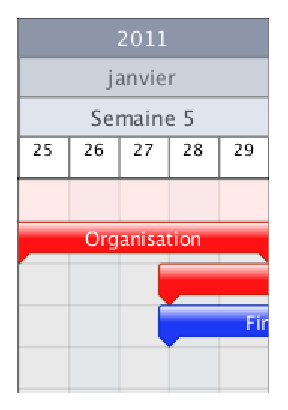
\includegraphics{./Organisation/Img/BomberBlok-Organisation.eps}
		\end{center}
	
	\subsection*{Conception}
		\begin{center}
			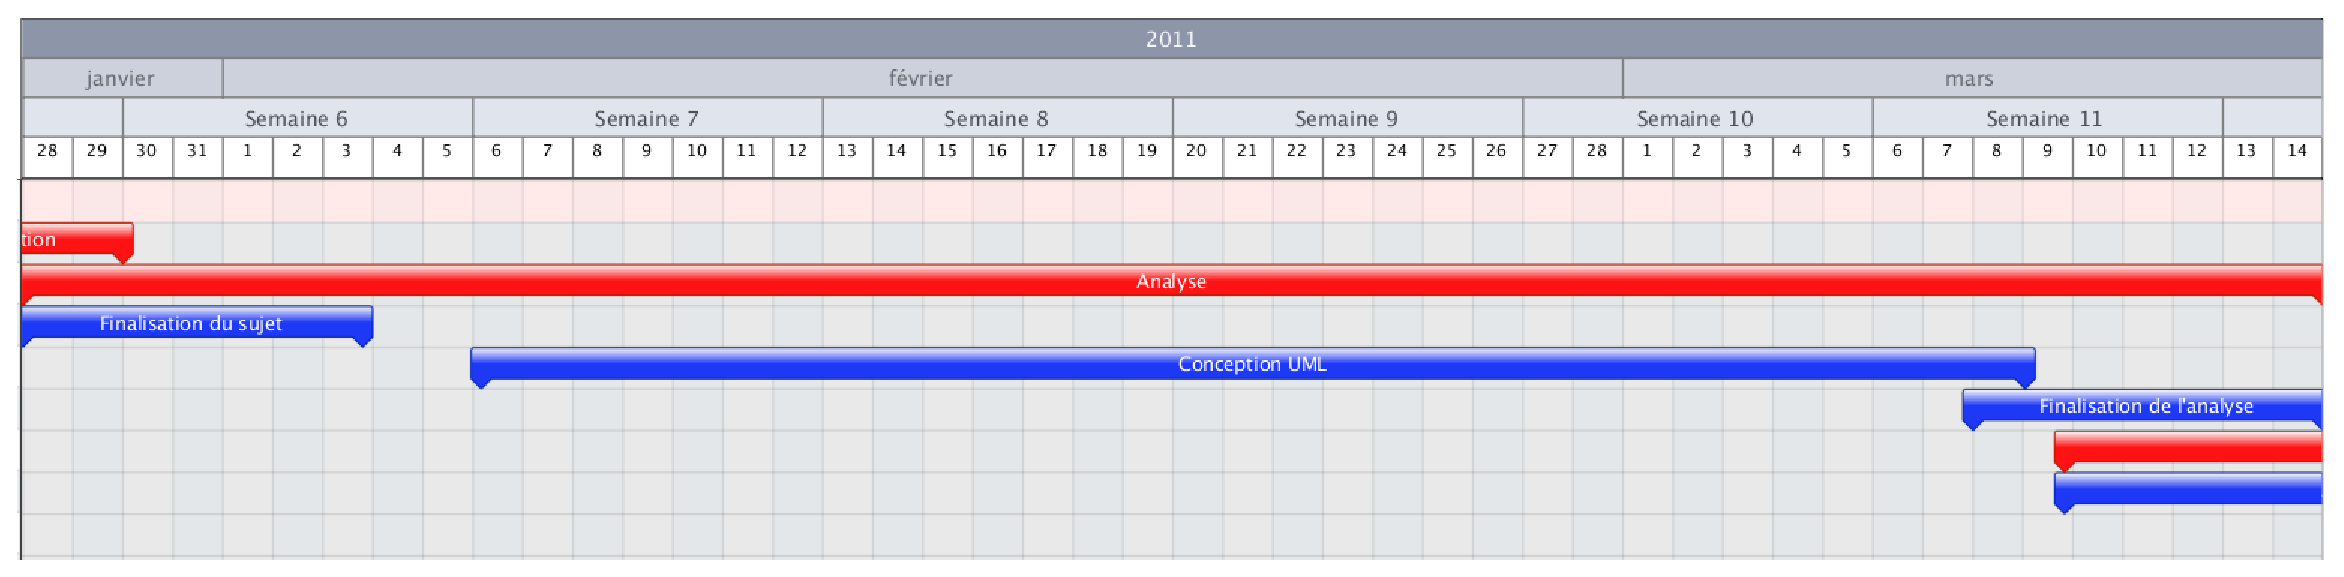
\includegraphics[width=20cm, angle=90]{./Organisation/Img/BomberBlok-Conception.eps}
		\end{center}
	
	\subsection*{Développement}
		\begin{center}
			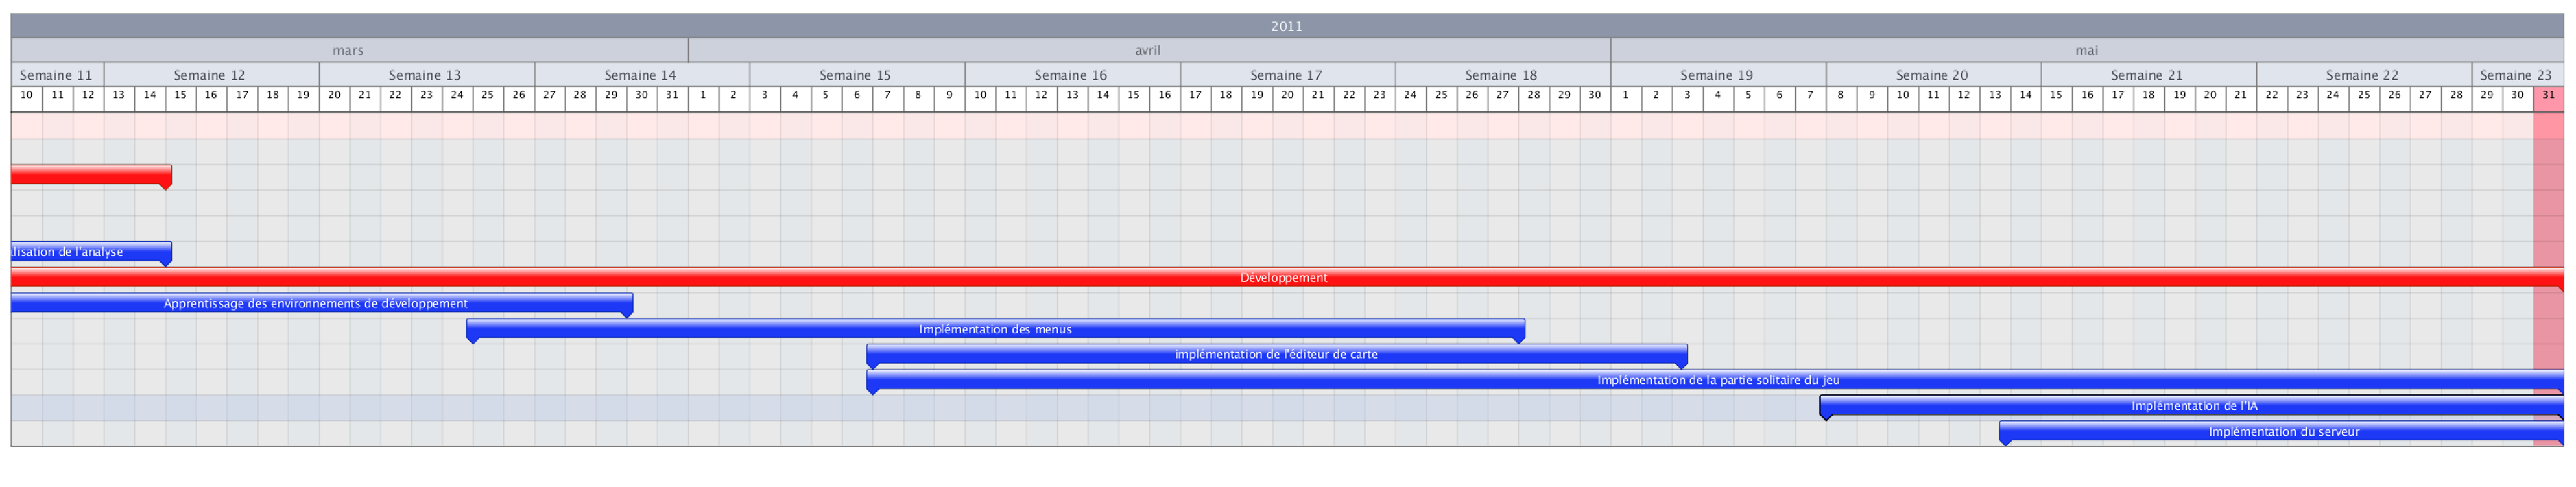
\includegraphics[width=20cm, angle=90]{./Organisation/Img/BomberBlok-Developpement.eps}
		\end{center}